\documentclass[14Q]{jsarticle}
\usepackage[dvipdfmx]{graphicx}
\usepackage{wrapfig}
\usepackage{float}
\usepackage{otf}
\usepackage{longtable}
\usepackage{ulem}
\usepackage{ascmac}
\usepackage{url}
\setlength{\textwidth}{160truemm}      % テキスト幅: 160mm
\setlength{\fullwidth}{\textwidth}     % ページ全体の幅
\setlength{\oddsidemargin}{0mm}   % 左余白
\setlength{\topmargin}{-10mm}       % 上余白
\setlength{\textheight}{240truemm}     % テキスト高さ: 297-(30+30)=237mm
\pagestyle{empty}
\title{北斗市二股台場の調査}% 文書のタイトル
\date{2018年12月3日}
\author{二股台場調査会 野村祐一,塚田直哉,石井淳平}              % 著者
%%%%%%%%%%%%%%%%
\begin{document}
\maketitle
%%%%
\begin{abstract}
北海道の南西部、北斗市の山中の台場山に、「二股台場」(北海道教育委員会埋蔵文化財包蔵地「台場山遺跡」(B-06-102))として知られる塹壕の跡が残されており、明治2年(1869)、鶉山道を越えて箱館五稜郭を目指す新政府軍との戦いに備えてここを守備した旧幕府軍が構築したと伝えられている。箱館戦争の戦跡としてだけではなく、城郭史研究の視点からも重要な遺跡である。

本調査ではこれまで知られている台場山周辺の塹壕群の測量を行い、塹壕群の形状と位置の記録を行った。今年度の調査では既知の17箇所の塹壕跡のうち5箇所と新発見の塹壕跡1箇所の測量調査を実施した。
\end{abstract}

%%%%
\section{二股台場の位置}
北斗市大野町市街地から約10km上流の大野川左岸に位置する。大野川とその支流である二股沢川の合流点付近に位置する。大野市街地から二股沢川付近までは大野川に沿って平坦な地形が続くが、二股台場塹壕群の所在する尾根を境に、これより上流では尾根と谷が交互に現れる急峻な地形となる。

二股台場塹壕群は二股沢川にと並行に北方から大野川にむかって傾斜する尾根上に位置する(図\ref{haiti})。標高261mの台場山と、これと一連の尾根をなす339m峰との間の尾根上に十数基の塹壕が確認されている。最高地点に立地する塹壕(F15)は標高約330m、最低地点に立地する塹壕(F16)は約200mである。尾根の鞍部を旧道である「鶉山道」が横切っており、塹壕群は鞍部をはさんで南北に分かれる。

新政府軍の攻撃正面となった尾根の西側斜面は鶉山道南側では平均傾斜約20度、鶉山道北側では約30度である。

\begin{figure}[h]
\centering
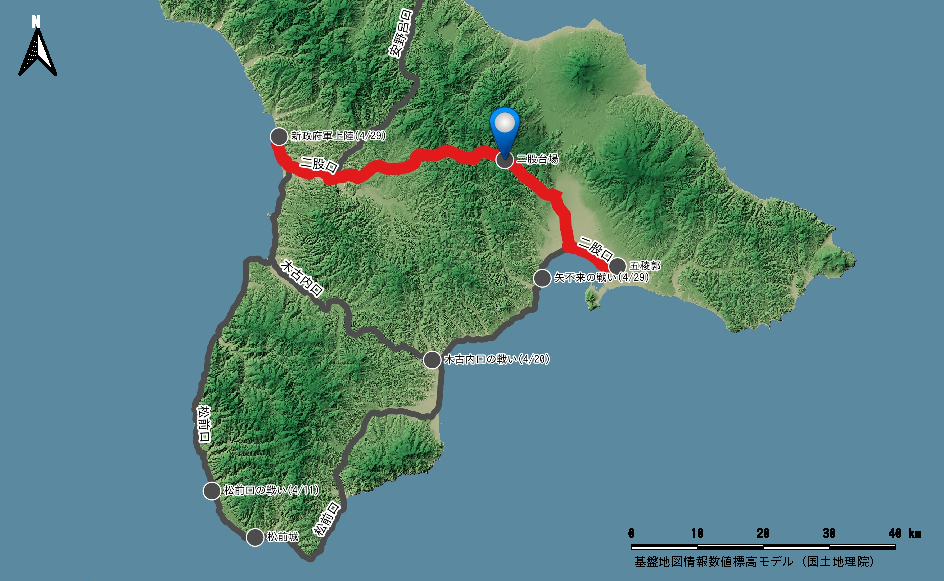
\includegraphics[width=160truemm]{fig/dounan.pdf}
\caption{二股台場の位置と明治2年箱館戦争}
\end{figure}

\begin{figure}[h]
\centering
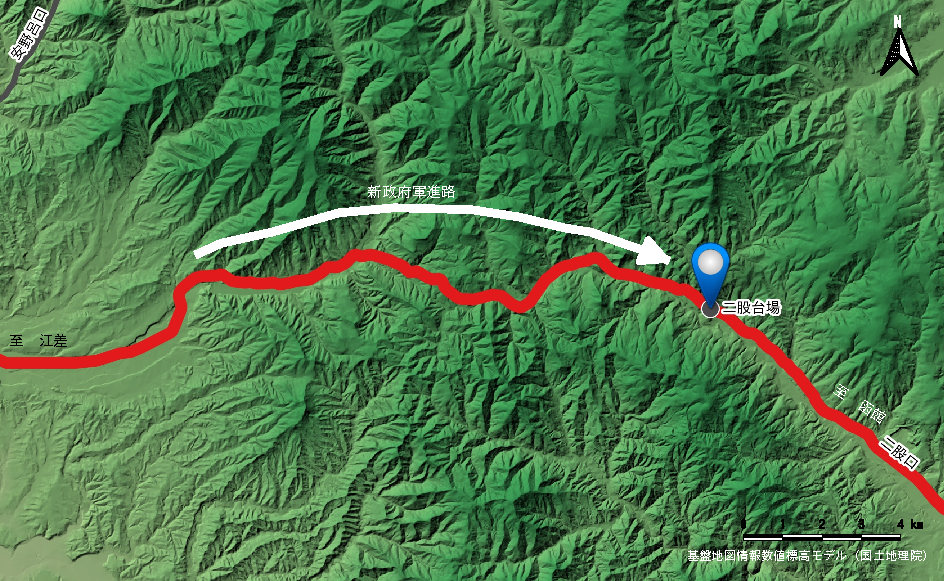
\includegraphics[width=160truemm]{fig/oonoassabu.pdf}
\caption{「鶉山道」と二股台場}
\end{figure}

\begin{figure}[h]
\centering
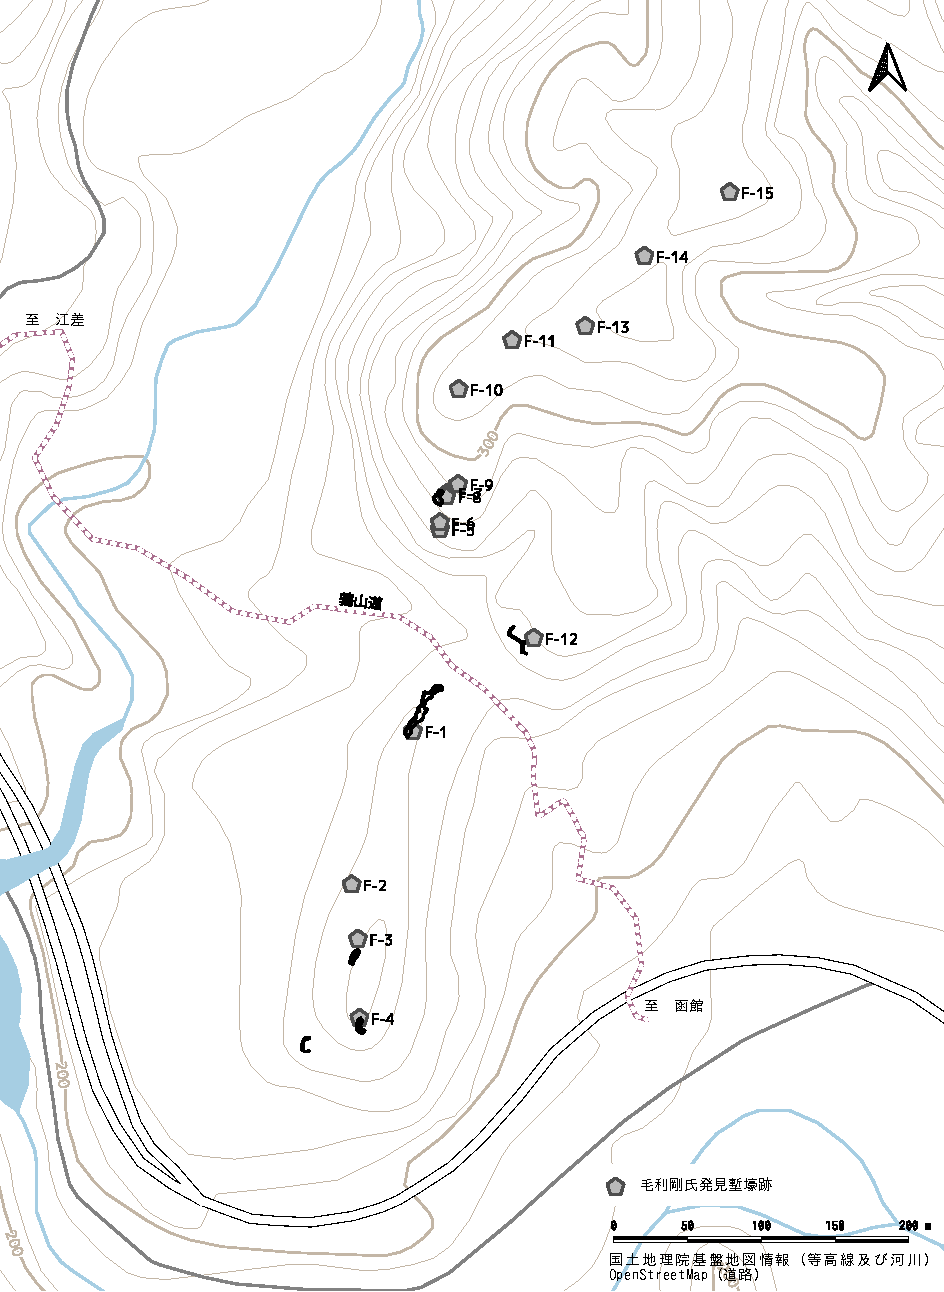
\includegraphics[width=160truemm]{fig/haitizu.pdf}
\caption{二股台場周辺の地形と塹壕配置}
\label{haiti}
\end{figure}

%%%%
\section{箱館戦争と二股台場}
\subsection{明治2年箱館戦争}
明治2年(1869)4月9日に北海道南西部の乙部に上陸した新政府軍は、ただちに西部の要衝である江差を占領した。新政府軍は「松前口」、「二股口」、「木古内口」、「安野呂ロ」の4つの攻撃軸を設定した。このうち、松前城のある「松前口」にもっとも大きな兵力が割かれており、ついで大きな兵力が派遣されたのが、現在の厚沢部町から北斗市を経由して箱館へ至る「二股口」である。

この動きを察知した旧幕府軍は、4月11日頃「台場山」に到着し、ここに陣地を構築する。『北国戦争概略衝鉾隊之記』によると、当初旧幕府軍は二股台場の対岸にあたる大野川右岸の「峠新道」に陣地を構築していたが、新政府軍が旧道を進むとの情報を得たため台場山に転陣したという。

\subsection{二股口の戦闘}
二股台場に対する新政府軍の攻撃は4月13日の夕方頃とされている(『北国戦争概略衝鉾隊之記』、『南柯紀行』)。二股台場から3kmほど西側の天狗岳付近にあった旧幕府軍の前進陣地に対する攻撃から、撤退する旧幕府軍を追って追撃戦がなされ、二股台場をめぐる攻防戦が開始された。戦闘は夜通し行われたとされるが、攻めあぐねた新政府軍は退却する。

2度めの戦闘は、4月23日の夕方頃とされる(前掲)。再び二股台場付近での戦闘となった。戦闘はこの日から翌々日の25日も夜通し続けられたが、二股台場からの逆襲を受けて新政府軍が敗走する場面もあり、二股台場の攻略に失敗した。26日早朝にはすべての新政府軍が二股台場周辺から撤退した。

\subsection{二股台場から退却}
その後、二股台場をめぐる大規模な戦闘は行われなかった。この間、松前口、木古内口での戦況は旧幕府軍にとって次第に悪化した。函館平野の入り口にあたる矢不来の防御戦闘が失敗に終わったことから、二股台場は戦略的な意味を失うこことなった。

4月29日、二股台場を守備していた旧幕府軍は陣地を放棄し、箱館五稜郭へ撤退した。守備隊の撤退により、二股台場は役割を終えることとなる。

%%%%
\section{研究史}
\subsection{河野常吉}
北海道庁の河野常吉による調査が大正12年に行われている。調査成果は翌大正13年の『北海道史跡名勝天然念物調査報告書』の中で報告されている。主な記載事項は次のとおりである。

\subsection{毛利剛氏の踏査}
2012年に塹壕の踏査とGPSによる位置記録、塹壕の略測図が作成された。調査成果については『二股口台場』(2012)としてまとめられ、F-1〜F-17までの17箇所の塹壕を記録している。

%%%%
\section{調査の方法}
\subsection{基準点と基線}
それぞれの塹壕に対して任意の基準点を設置した。基準点はハンディGPS(Garmin社製etrex20J)を用いて座標を計測した。座標計測に際しては、基準点に5分以上設置し平均値を測定した。

基準点から、遺構測量に適当な方向に基準線を設定し、これを基線として平面図を作成した。平面図には登山用のコンパスで測定した磁北を記入した。

%%%%
\subsection{実測の方法}
現地での測量図は20分1を原則とし、F01では100分1で作図した。

%%%%
\subsection{GISでの作図}
現地測量図は以下の手順でデジタル化しGISデータを作成した。投影系・座標系は「JGD2000UTMzone54」である。
\begin{enumerate}
\item 現地での測量図をもとに素図を作成した。
\item これをA3版に縮小して200dpiでスキャンした。
\item スキャン画像をQGISに取り込み幾何補正を行った。
\item 幾何補正された遺構図をQGIS上でトレースしベクタデータを作成した。
\end{enumerate}

%%%%
\subsection{LocalWikiを使用した調査状況の公開}
本調査については、調査中からLocalWiki\footnote{
地域に関する記事を集積するウェブプラットフォーム。クリエイティブ・コモンズライセンス 表示による公開が原則である。誰でも自由に新しいWiki(リージョン)を立ち上げて編集することができる。
}
にリージョン「北斗市二股台場」(\url{https://ja.localwiki.org/futamata/})を開設し、調査状況や遺構配置図、関連資料について掲載してきた。

%%%%
\subsection{GitHubを使用した調査データの公開}
調査に関する写真、図面、GISデータはGitHub\footnote{
Gitはバージョン管理システムの一種で複数ユーザーによるデータ更新の履歴を管理することを目的とする。GitHubはGitの仕組みを利用したウェブサービスで、ウェブ上にあるリモートリポジトリは公開が原則となる。
}
(\url{https://github.com/IshiiJunpei/Futamata})で管理・公開している。GitHubを利用するメリットは、調査データの管理と公開を同時に行うとともに、データの変更履歴がすべて記録されるため、改ざん行為が原則的に不可能となる点である。

また、調査の成果を汎用性の高いGISデータ\footnote{
GISデータは.gpkg(Geopackages)形式で保存した。
}
とすることで環境に依存せずに調査成果の再利用が可能となっている。

%%%%
\section{調査の経過}
\subsection{2017年11月5日}
\begin{itemize}
\item 調査内容 F01塹壕の測量調査
\item 調査者  石井淳平
\end{itemize}

\subsection{2018年4月28日}
\begin{itemize}
\item 調査内容 F03、F04、F18塹壕の測量調査。F02塹壕は発見できなかった。
\item 調査者  野村祐一、石井淳平、石井遼平
\end{itemize}

\subsection{2018年5月26日}
\begin{itemize}
\item 調査内容 F08、F12塹壕の測量調査及び鶉山道北側高所の塹壕群の位置把握を行った。F07、F09、F10、F11、F13、F15を確認することができたが、F05、F06、F07、F14については発見できなかった。
\item 調査者  野村祐一、塚田直哉、石井淳平
\end{itemize}

%%%%
\section{塹壕配置}
図\ref{haiti_tate}に示すように、塹壕群は鶉山道で南北に分断される。もっとも長大なF01塹壕は鶉山道の南側で山道に北端を接している。山道北側の塹壕群が山道を見下ろす位置にあり山道の北側側面に面して配置される。339m峰に近い尾根の高所にもF10、F11、F13、F15塹壕が配置される。

\begin{figure}[h]
\centering
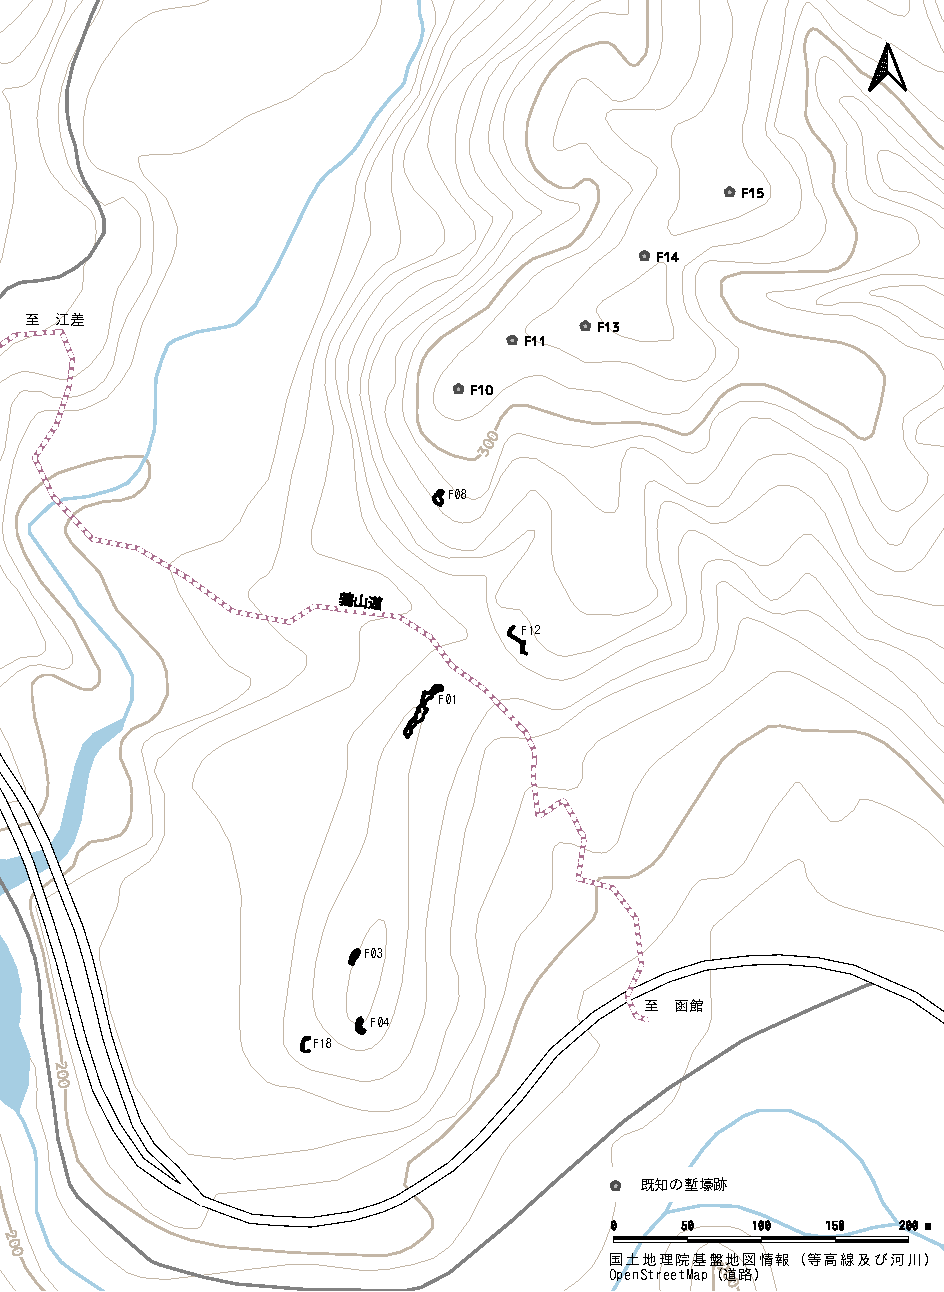
\includegraphics[width=160truemm]{fig/haitizu_tate.pdf}
\caption{塹壕配置}
\label{haiti_tate}
\end{figure}

%%%%
\section{塹壕}
\subsection{F01(図\ref{f01})}
「イナズマ型塹壕」として知られる塹壕である。二股台場塹壕群中もっとも延長が長く30mを超える。「イナズマ」の由来となった塹壕の屈曲については平面図上では明瞭ではなく、意図的な屈曲というよりも、地形にそって塹壕が構築されたためジグザグにみえるようである。また、毛利剛(2012,p10)が指摘するように河野常吉(1924)の調査ではこのような長大な塹壕は確認されていないことから、複数の塹壕が見学者の踏み跡によってつながって見えるようになってしまった可能性がある。X=4643830ライン付近は意図的な突出部と考えられる。

\begin{figure}[h]
\centering
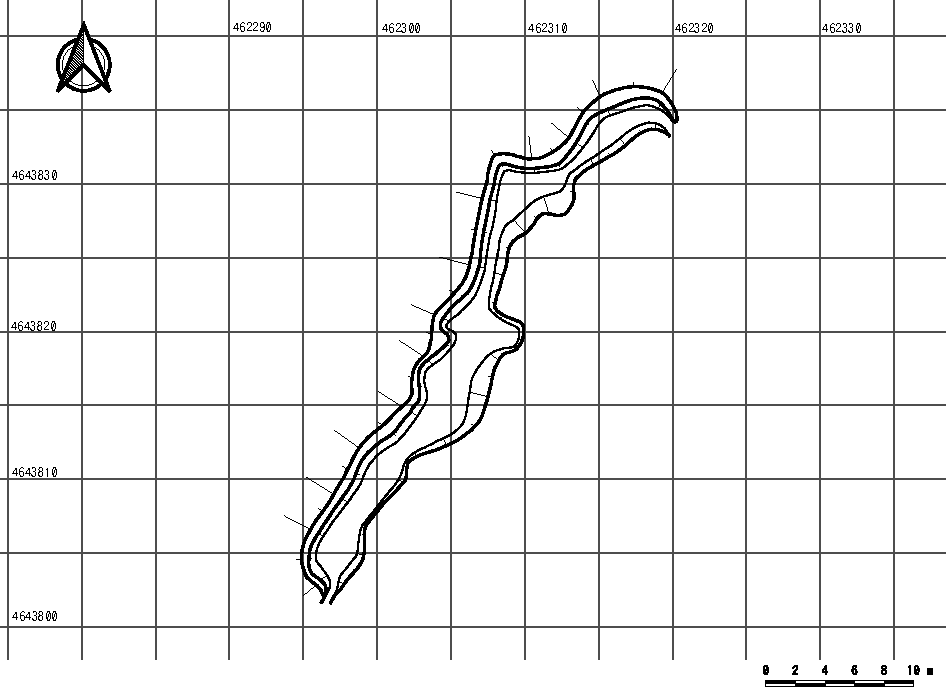
\includegraphics[width=160truemm]{fig/F01.pdf}
\caption{F01塹壕}
\label{f01}
\end{figure}

%%%%
\subsection{F03塹壕(図\ref{f03})}
F01塹壕南西、直線距離で約150m離れた尾根の先端付近に位置する。毛利剛氏の踏査ではF01塹壕とF03塹壕の間にF02塹壕が確認されているが、今回の調査では発見できなかった。長軸は北東-南西方向で長さ約10mである。

\begin{figure}[h]
\centering
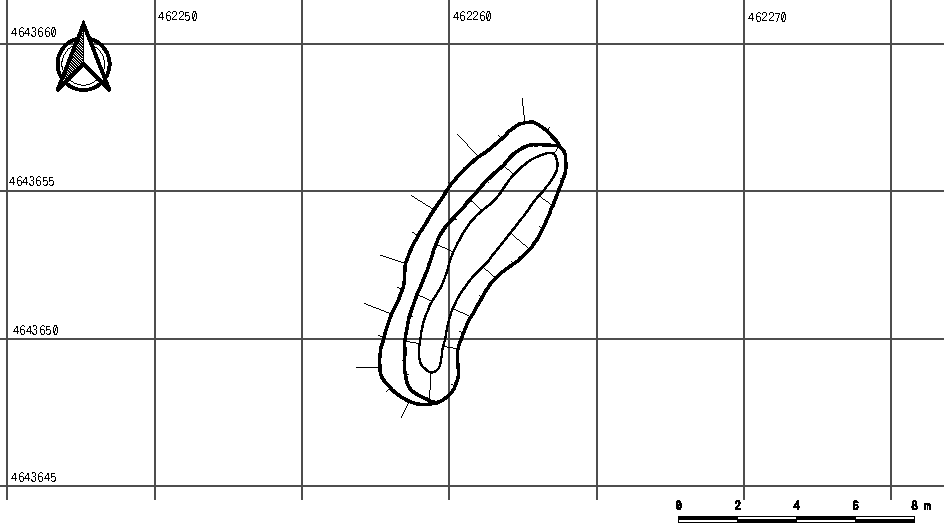
\includegraphics[width=160truemm]{fig/F03.pdf}
\caption{F03塹壕}
\label{f03}
\end{figure}

%%%%
\subsection{F04塹壕(図\ref{f04})}
F03から南に約40mのところに位置する。尾根の先端に構築される。長軸は南北方向で約10mである。

\begin{figure}[h]
\centering
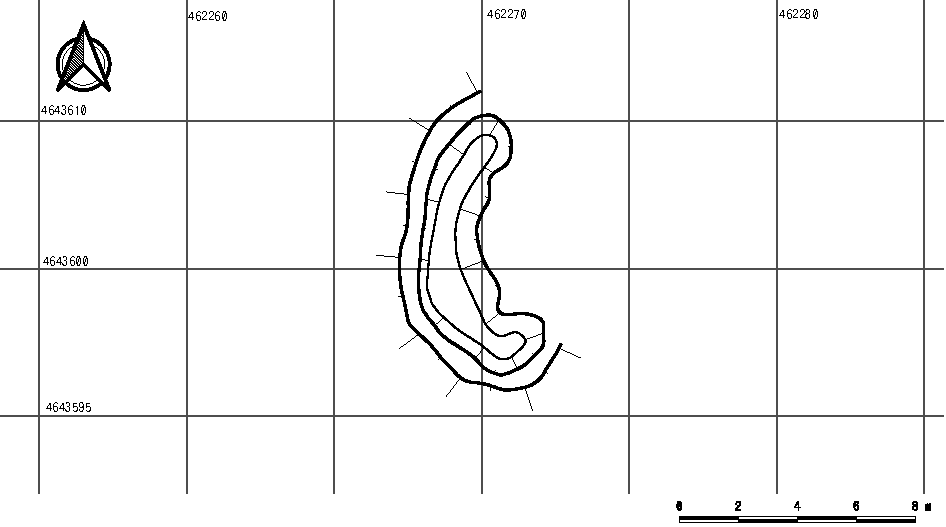
\includegraphics[width=160truemm]{fig/F04.pdf}
\caption{F04塹壕}
\label{f04}
\end{figure}

%%%%
\subsection{F18塹壕(図\ref{f18})}
新発見の塹壕である。F04から南東に約35mのところに位置する。尾根の先端にむかう傾斜面に構築される。長軸は南北で長さ約10mである。斜面を削り出して幅4m、長さ8mの平坦地を形成する。

\begin{figure}[h]
\centering
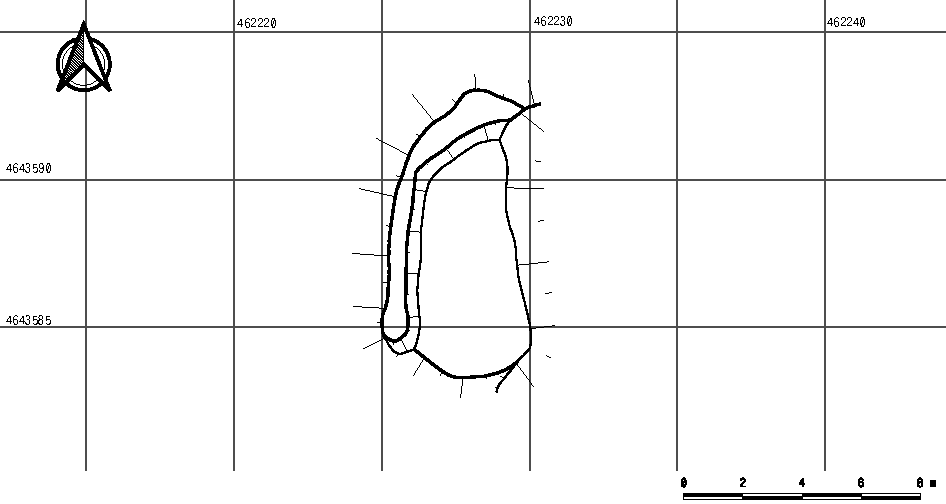
\includegraphics[width=160truemm]{fig/F18.pdf}
\caption{F18塹壕}
\label{f18}
\end{figure}

%%%%
\subsection{F12塹壕(図\ref{f12})}
鶉山道北側で最も鶉山道に近い位置に位置する。鶉山道を挟んでF01塹壕がある。北東-南西方向の斜面に構築される。塹壕の掘り込みは不明瞭で土塁はクランク状に2度屈曲する。土塁の延長は約20mである。

\begin{figure}[h]
\centering
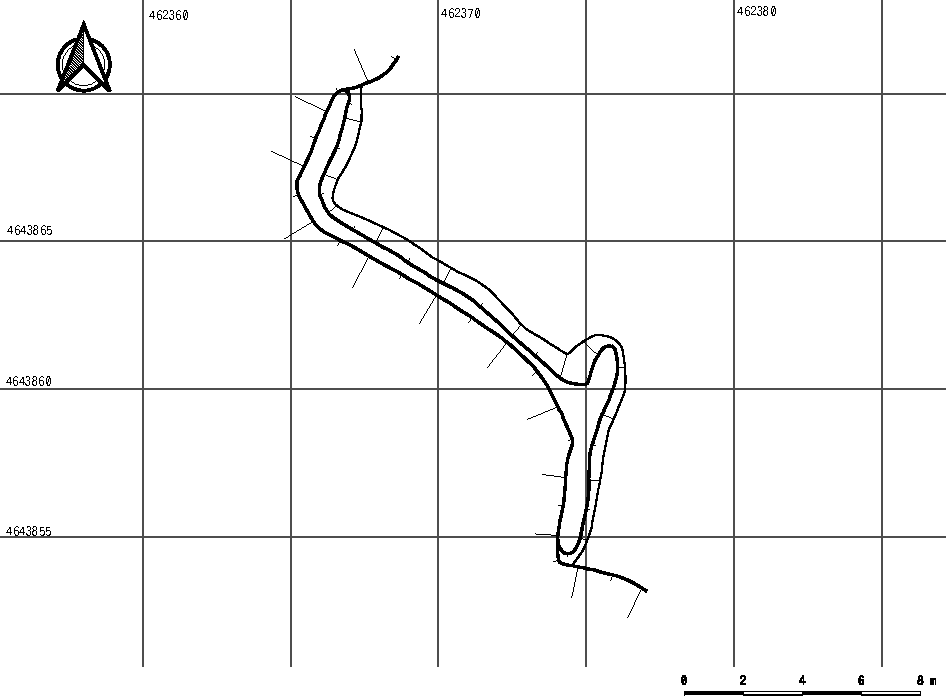
\includegraphics[width=160truemm]{fig/F12.pdf}
\caption{F12塹壕}
\label{f12}
\end{figure}

%%%%
\subsection{F08塹壕(図\ref{f08})}
F12塹壕から北西に約100mのところに位置し、F12からは小さな沢を挟んだ尾根上に立地する。約30度の斜面に構築される。南側は斜面を削り込んで幅約3mの平坦面をつくりだす。

\begin{figure}[h]
\centering
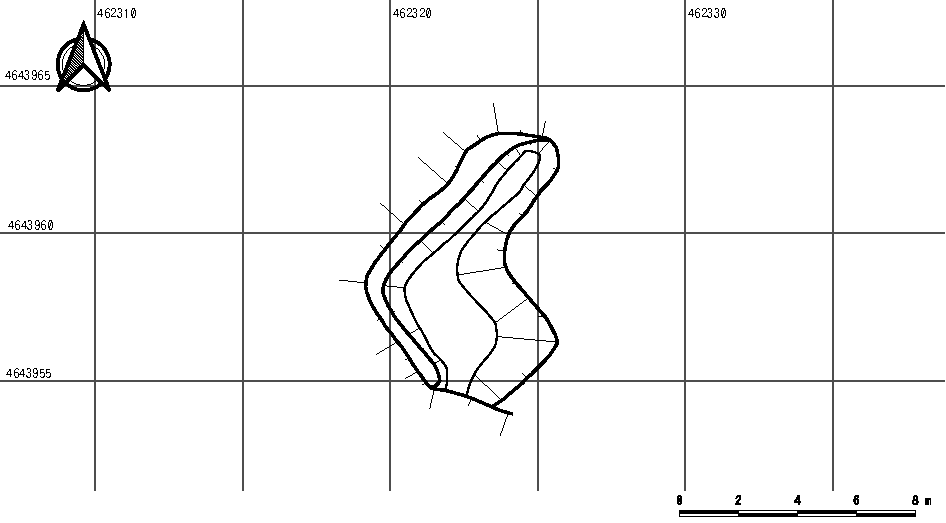
\includegraphics[width=160truemm]{fig/F08.pdf}
\caption{F08塹壕}
\label{f08}
\end{figure}

%%%%%
\section{まとめ}
\subsection{立地の特徴}
二股台場は大野川の中流域から上流域の境界付近に立地する。二股台場より上流では大野川は蛇行を繰り返し、尾根と谷が連続する地形となり、大野川沿いに通行することは困難となる。一方、二股台場より下流では大野川の氾濫原が広がり大野川沿いに歩行することが可能となる。二股台場は、江差方面に対しては急峻な地形となり、箱館方面に対してはなだらかな地形となる地形の境界に立地する。

二股台場の所在する台場山及び339m峰の尾根は大野川に対して大きく南側へ張り出しており、「鶉山道」は台場山と339m峰の鞍部を通過する。二股台場は鞍部を通過する鶉山道を遮断する南北方向に塹壕が構築される。

二股台場の立地の特徴については次のようにまとめることができる。

\begin{enumerate}
\item 大野川上流の急峻な地形を利用しつつ、箱館方面からの補給や連絡が容易な地点を選定している。
\item 鶉山道を遮断することを目的とした選地と塹壕配置となっている。
\end{enumerate}

%%%%
\subsection{塹壕配置(図\ref{view})}
\paragraph{鶉山道南側塹壕群}
二股台場の塹壕群のうち、鶉山道南側の台場山に構築された塹壕群は等高線と並行に構築され、西側あるいは南側に土塁を設ける構造となっている。主たる防御方向である台場山西斜面は傾斜角度20度前後の比較的緩やかな斜面が広がる。手を使わずに登攀できる傾斜であり、F01、F03、F04、F18の「鶉山道南側塹壕群」は攻撃の脅威に晒される西と尾根の先端方向の東に対して土塁を配備している。

\paragraph{鶉山道北側低位塹壕群}
一方、鶉山道北側の339m峰へつづく尾根に構築された塹壕群のうちF08、F09、F12の「鶉山道北側低位塹壕群」は西側だけではなく、鶉山道のある南側にも土塁を設けている。339m峰へつづく尾根の西側斜面は傾斜角度40度を超える急傾斜面が連続し、ここを登攀することはきわめて困難であることから、西側斜面に対しては大きな脅威が存在しなかったと考えられる。先述したように、台場山西側斜面はゆるやかであり、西側からの攻撃の脅威にさらされやすい。こうしたことから、339m峰へつづく尾根に構築されたF08やF12などは西側に土塁を築くとともに南側にも土塁を構築し、鶉山道に対して側面からの攻撃や「鶉山道南側塹壕群」の支援を可能にする塹壕構造となっている。

\paragraph{鶉山道北側高位塹壕群}
鶉山道北側の339m峰に近いF10、F13、F14、F15の「鶉山道北側高位塹壕群」からは鶉山道を直接視認することはできない。西側の二股川対岸を視界に入れ、西側に対して備えた塹壕構造となっている。

二股台場の塹壕配置については次のようにまとめることができる。

\begin{enumerate}
\item 西側に緩斜面が広がる「鶉山道南側塹壕群」は西側に土塁を備え、西側を強く意識した構造をもつ。
\item 西側に急斜面がある「鶉山道北側低位塹壕群」は、西側と南側に土塁を備え、西側に対する防衛とともに、南側の鶉山道の側面攻撃や「鶉山道南側塹壕群」を側面から支援することを意識した構造をもつ。
\item 339m峰に近い「鶉山道北側高位塹壕群」は、鶉山道よりも二股川対岸の新政府軍陣地に対して備えた構造をもつ。
\end{enumerate}

\begin{figure}[h]
\centering
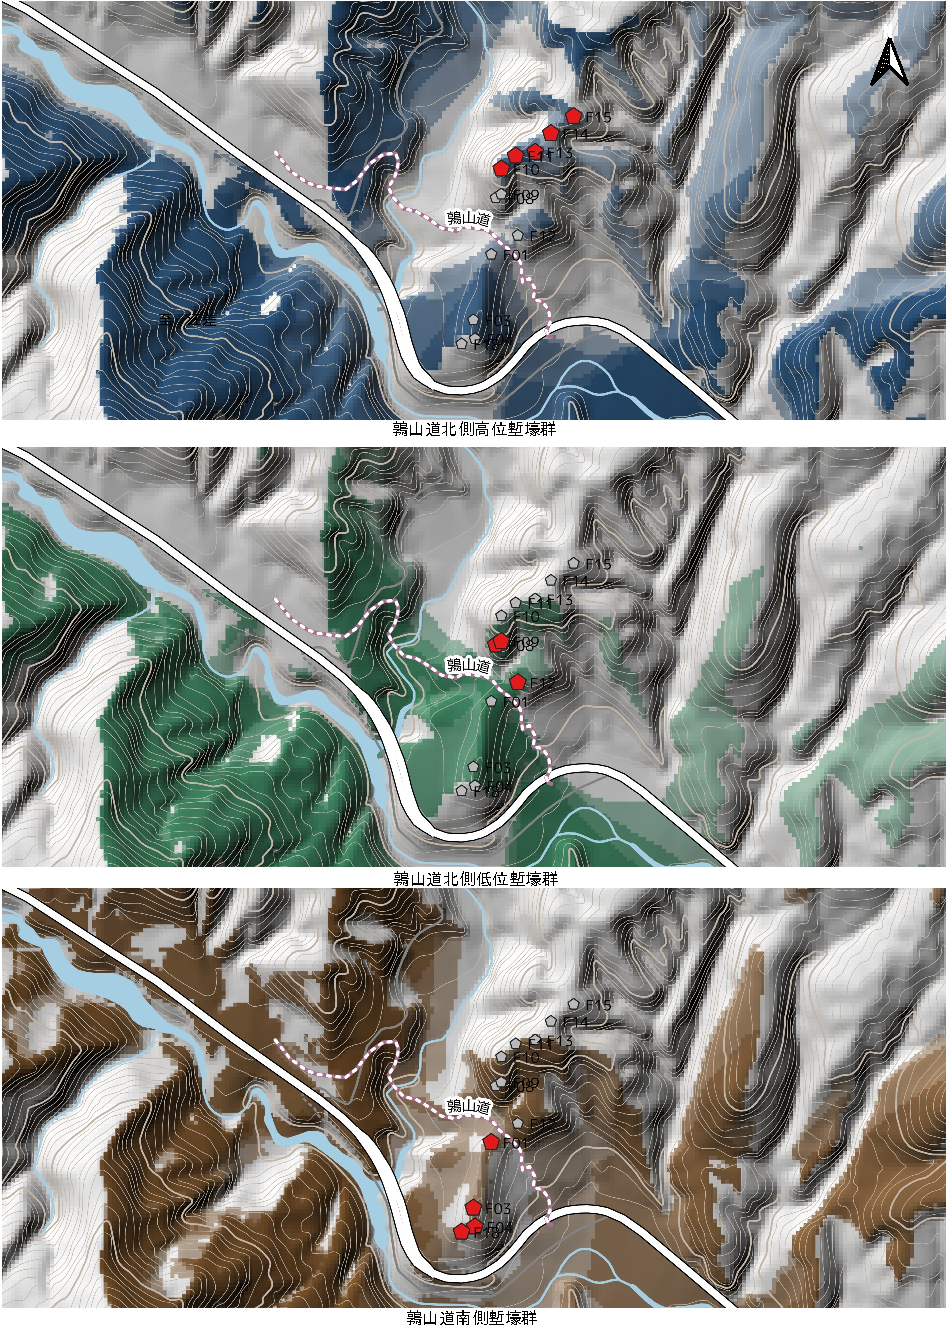
\includegraphics[width=160truemm]{fig/view.pdf}
\caption{二股台場塹壕群の可視領域}
\label{view}
\end{figure}

%%%%
\section{今後の調査}
2018年の調査ではこれまで知られている17基の塹壕のうち、6基の測量調査を行った。2019年は未確認の塹壕の確認と測量調査を進めるとともに、未作成の横断図の作成を行う。


\section*{参考文献}
\noindent
今井信郎『北国戦争概略衝鉾隊之記』,1998『南柯紀行・北国戦争概略衝鉾隊之記』新人物往来社,pp.159-184\\
今井信郎『蝦夷之夢』,1998『南柯紀行・北国戦争概略衝鉾隊之記』新人物往来社,pp.186-228\\
今井信郎『衝鋒隊戦争略記』,須藤隆仙編著 1996『箱館戦争史料集』新人物往来社,pp.80-86\\
大鳥圭介『南柯紀行』,1998『南柯紀行・北国戦争概略衝鉾隊之記』新人物往来社,pp.230-258\\
河野常吉 1924『北海道史蹟名勝天然記念物調査 大正拾一年』,北海道立図書館所蔵,pp.-\\
毛利 剛 2012『二股口台場』自遊出版工房



\end{document}
